\documentclass[conference]{IEEEtran}
\IEEEoverridecommandlockouts
% The preceding line is only needed to identify funding in the first footnote. If that is unneeded, please comment it out.
\usepackage{cite}
\usepackage{amsmath,amssymb,amsfonts}
\usepackage{multicol}
\usepackage{algorithmic}
\usepackage{graphicx}
\usepackage{textcomp}
\def\BibTeX{{\rm B\kern-.05em{\sc i\kern-.025em b}\kern-.08em
    T\kern-.1667em\lower.7ex\hbox{E}\kern-.125emX}}
\begin{document}

\title{SIMD Acceleration for Index Structures\\
}

\author{\IEEEauthorblockN{Marten Wallewein-Eising}
\IEEEauthorblockA{\textit{Otto-von-Guericke University} \\
Magdeburg, Germany \\
marten.wallewein-eising@st.ovgu.de}
}

\maketitle

\begin{abstract}
\begin{itemize}
	\item summary: 
	\subitem Give short an overview of SIMD and modern index structures
	\subitem Explain what are the problems of the ``old" index structures made for disk-based database systems
	\subitem Explain which approaches were made to adapt index structures to modern systems and what they have in common and what are differences
	\item Why is this work important: 
	\subitem Give a state of current development of the index structures
	\subitem Collect common approaches to adapt other index structures TODO: ReThink
	\item K-ary search trees, FAST, VAST and ART compared
	\item Contribution: What are important approaches used by different implementations to adapt index structures to modern systems
\end{itemize}
\end{abstract}

\begin{IEEEkeywords}
SIMD, index 
\end{IEEEkeywords}

\section{Introduction}
% Main Problem: Index structures designed for disk-based database systems
After decades of creating and improving index structures for disk-based database systems, nowadays even large databases fit into the main memory. Since index structures like the $B^+$-tree or the radix tree have an important part in database systems to realise scan or range-based search operations, these index structures experienced many adaptions to fulfill the needs of modern database systems. Instead of overcoming the bottleneck of IO-oprations from disk to RAM, the target of modern index structures is to improve the usage of CPU cache and processor architectures.

% Introduce tree structures and specific Problem: Cache and TLB misses and branch mispredictions cost a lot of calculation effort
Several index structures have already shown that the bottleneck from RAM to CPU can be overcome using Single Instruction Multiple Data (SIMD) [1] operations. These index structures include: the K-ary Search Tree (Seg-tree) [3], Adapted Radix Tree (ART) [4], Fast Architecture Sensitive Tree (FAST) [6], and Vector-Advanced and Compressed Structure Tree (VAST) [5]. As the authors of VAST-Tree show, important causes for increased runtime are cache misses and branch mispredictions. To overcome branch mispredictions and to decrease CPU cycles, SIMD  is used in modern index structures for tree traversal [2]. The authors of the k-ary search show how to use SIMD to compare mutliple keys in one CPU cycle. To decrease cache misses, the authors of FAST and ART show how to adapt index structures to the cache line size.  

% Objectives and Contribution
%TODO: Rewrite, all approaches use SIMD but in different ways, therefore difficult to compare...
\textbf{TODO: Fix!} All approaches use SIMD only for key comparison within tree traversal and try to decrease the key size to fit more keys into one SIMD register. Therefore FAST and Seg-tree only provide implementations for search algorithms. We consider the design approaches of VAST and ART to implement operations like update and insert und name ideas to use SIMD for them. Consequently, with this work we make the following contributions:
\begin{itemize}
	\item We compare different adaptions of index structures to fulfill requirements of modern database systems
	\item We highlight the usage of SIMD and the cache line adaptions in all approaches
	\item We show opportunities for adaption for other approaches to use SIMD
\end{itemize}
% Paper structure
We organized the rest of the paper as follows. In Section 2, we give the preliminaries for SIMD in general and for the use in index structures. In Section 3, we analyse the different approaches of adapted index structures and evaluate the comparision in Section 4. In section 5, we name related work. In Section 6, we present our conclusion und describe future work in Section 7. 
\section{SIMD-Style Processing}
\begin{figure}
	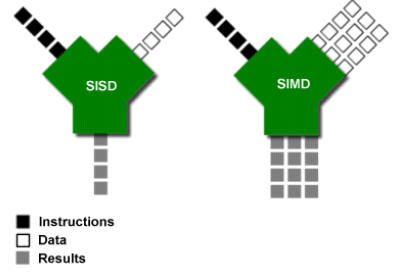
\includegraphics[width=0.4\textwidth]{figure_1.png}
	\caption{Coherence between data, instructions, and the results of SISD and SIMD.}
	\label{fig}
\end{figure}
% SIMD explanation
A common approach of decreasing CPU cycles for algorithms is to adapt the algorithm to pipelining. While one instruction is executed, the next instruction is already fetched. This approach executes one instruction on one data item, called Single Instruction Single Data (SISD). In contrast to execute one operation on one data item after another, the idea of SIMD is to execute a single instruction on multiple data. In Figure 1 we show the coherence between data, instructions, and the results of SIMD and SISD. 
\begin{table*}[htbp]
	\caption{SIMD instructions from Streaming SIMD Extensions 2 (SSE2) TODO: Maybe add some more :)}
	\begin{center}
		\begin{tabular}{|c|c|}
			\hline
			\textbf{SIMD instruction}&\textbf{Explanation}\\
			\hline
			\_\_m128i \_mm\_load\_si128 (\_\_m128i *p) & Loads a 128-bit value. Returns the value loaded into a variable representing a register.\\
			\_\_m128i \_mm\_cmpgt\_epi32 (\_\_m128i a, \_\_m128i b) & Compares 4 signed 32-bit integers in a and 4 signed 32-bit integers
			in b for greater-than.\\
			\hline
		\end{tabular}
		\label{tab1}
	\end{center}
\end{table*}
% SIMD explanation
Modern CPUs have additional SIMD registers along with an additional instruction set adapted to process multiple data items in parallel. In Table 1, we show some SIMD instructions from Streaming SIMD Extensions 2 (SSE2). We consider \_mm\_cmpgt\_epi32 as example to show how SIMD works.\textbf{TODO: fix Example, $a > b$} After loading 4 different signed 32-bit integers in a and 4 equal signed 32-bit integers in b, we compare them using \_mm\_cmpgt\_epi32. The comparision returns a bitmask showing which of the search keys in a is greater than the one in b. This example increases the performance of comparision by times of four. 

% Pro's/contra's of SIMD
Consequently, the main advantage of SIMD is to process multiple data parallel in contrast to pipelining and SISD. The main restriction of SIMD instructions is that a sequential load of data is required. To load data into a SIMD registert, the data has to be stored consecutively in main memory. Additionally, the size of SIMD registers is limited. Therefore processing data types of the common size of 64-bit and more lead to a small performance increase since only few data items are processed with a single instruction.

% Horizontal vs vertical vector processing
Polychroniou et al. [7] show two general approaches to use SIMD in in-memory databases, horizontal and vertical vector processing. They name the comparision of one search key to multiple other keys horizontal vectorization, whereas processing a different input key per vector lane is named vertical vectorization.

% How horizontal vectorization works
Since FAST, Seg-Tree, ART and VAST only use horizontal vectorization, we focus on this approach.  For example, Zeuch et al. [3] use 128-bit SIMD registers and adjusted SIMD operations to load data into a register and to compare the data of one SIMD register with another. A 128-bit SIMD register processes sixteen 8-bit or eight 16-bit data items with one instruction. In Table 2 TODO: Insert Table! we show a comparision of key size and the number of keys that can be processed parallel with one SIMD instruction.

% SIMD restrictions

%TODO: Figure over 2 columns, include lipsum/multicol packe 
\section{Adapted Tree Structures}
% TODO: Compare all 4 or merge FAST and VAST together/ extend FAST with VAST??
In this section we present the previously mentioned index structures Seg-Tree, FAST, ART, and VAST. We consider the adaptions made compared to the base index structure, the usage of SIMD, and the performance gain presented by the authors of the certain index structures.
\subsection{Seg-Tree}\label{SCM}
% Basics k-ary search
Zeuch et al. adapted the $B^+$-Tree by having a k-ary search tree as each inner node, called segment, and perform a k-ary search on each segment.  In Figure 2, we show the adaption of nodes made by Zeuch et al. for Seg-Tree. The k-ary search bases on the binary search but divides the search space into k partitions with k-1 seperators. Compared to binary search the k-ary search reduces the complexity from $O(\log{2}{n})$ to $O(\log{k}{n})$. They consider $m$ as the most bits to represent a datatype and $\vert SIMD \vert$ as the size of SIMD-register, called SIMD bandwith. Then, $k = \frac{\vert SIMD \vert }{m}$ defines the number of partitions for the k-ary search. 

\begin{figure}
	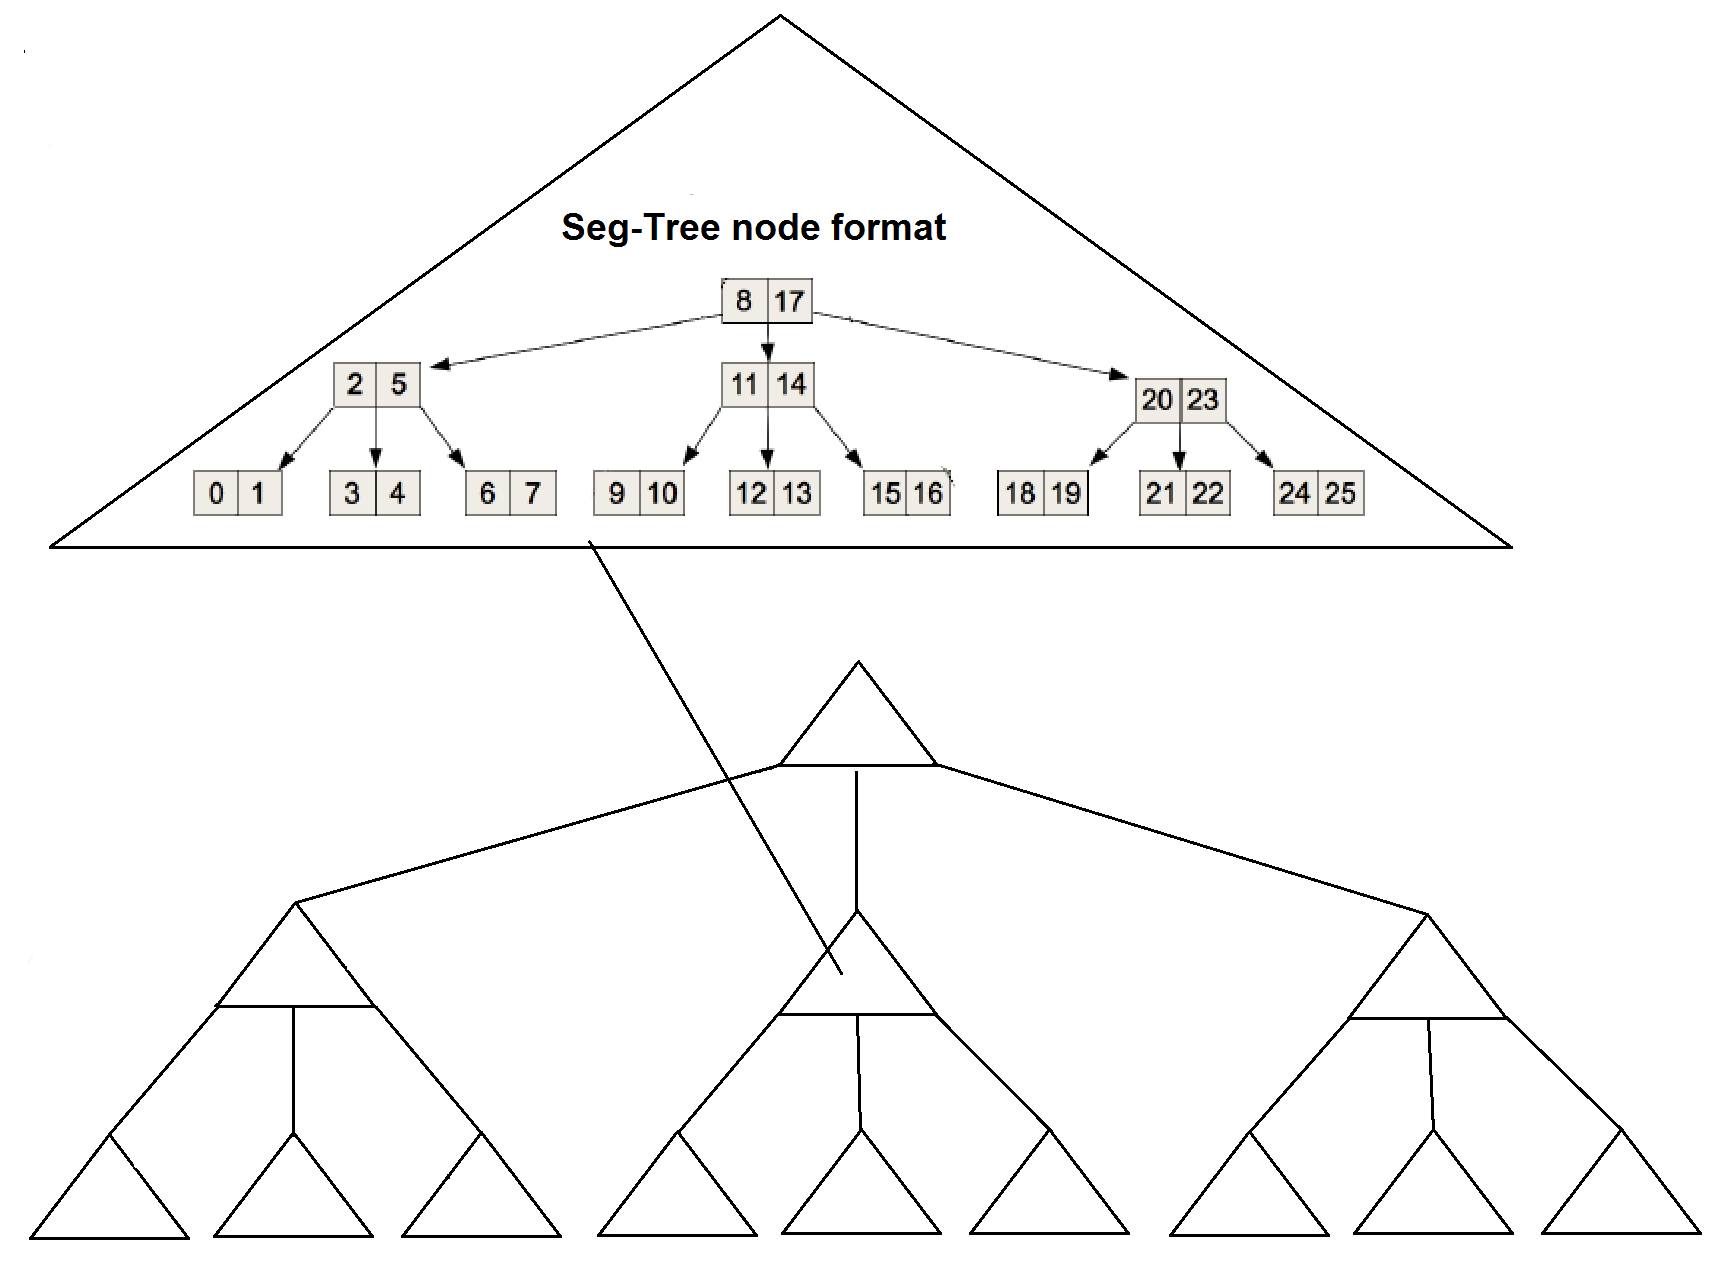
\includegraphics[width=0.5\textwidth]{figure_2.png}
	\caption{Inner node format of Seg-Tree}
	\label{fig}
\end{figure}

% Performing k-ary search on Seg-tree
As mentioned before, each segment of the Seg-Tree is a k-ary search tree. To perform a k-ary search on a segment, Zeuch et al. linearize the elements of the segment. They show two algorithms for linearization, breadth-first search and depth-first search. Because of the condition $k = \frac{\vert SIMD \vert }{m}$, each partition of the k-ary search fits into a SIMD register and is compared to the search key. A perfect k-ary search tree contains  $S_{max} = k^h - 1$ keys for an integer $h > 0$. The considered search algorithm only works for sequences with a multiple of $k-1$ keys. In case of  sequences with less than a multiple of $k-1$ keys, they replenish the sequence with elements having the value $k_{max} + 1$ for the maximal key value $k_{max}$ in the sequence. Consequently, the adapted search algorithm works for sequences with less than a multiple of $k-1$ keys.

% Performance increase
The performance of Seg-Tree depends on k-ary search. The smaller a key the more keys are compared parallel. According to the relevance of 32 and 64-bit data types in modern systems, the k-ary search performance increases only by the factor of four for 32-bit types and two for 64-bit types.

\begin{figure*}
	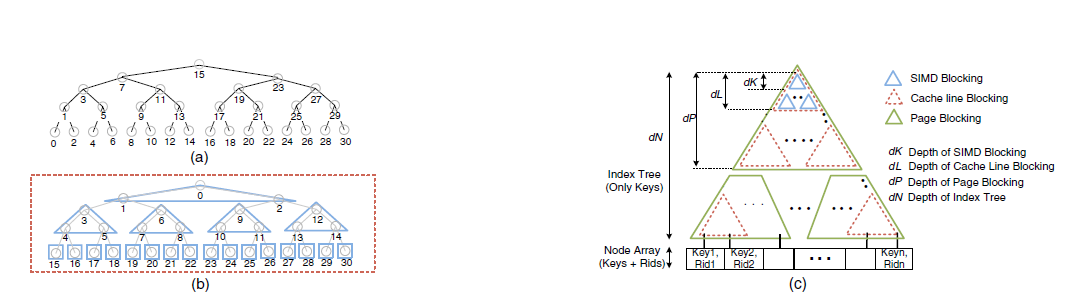
\includegraphics[width=1.0\textwidth]{figure_3.png}
	\caption{(a) Node indices (=memory locations) of the binary tree (b) Rearranged nodes with SIMD blocking (c) Index tree blocked in three-level
		hierarchy – first-level page blocking, second-level cache line blocking, third-level SIMD blocking. Adapted from Zeuch et al. [3].}
	\label{fig}
\end{figure*}

% Addional adaption: Seg-trie
%TODO: Each Node is also k-ary search tree
Zeuch et al. also show the k-ary search on an adapted prefix tree \emph{(trie for short)} called Seg-Trie. A trie is a search tree where each node stores a part of the key. Each node is again designed as a k-ary search tree. Complete keys are stored in leaf nodes or are build by concatenating partial keys from the root node to a leaf node. This approach benefits of the separation of the keys in different levels of the tree. Consequently, the compare keys are smaller and more keys can be compared in parallel. The Seg-Trie$_L$ is defined as a balanced trie where each node on each level contains one part of the key with $L$ Bits. The tree has $r = \frac{m}{L}$ levels $(E_0, E_1, .., E_r)$, where m is the number of most bits to represent the data type.

% K-ary search on Seg-Trie
To perfom a tree traversal on the seg-trie, the search key is split into $r$ segments and each segment $r_i$ is compared to the level $E_i$. If a matching partial key is found in one node of $E_i$, the search continues at the referrenced node for the partial key. If no match of the partial key is found, the Seg-Trie does not contain the search key and the search is finished. Consequently, the advantage of Seg-Trie against tree structures is the reduced comparision effort for non-exisiting key segments. 

% Performance increase of Seg-Trie?

\subsection{FAST}\label{SCM}
% Introduction of FAST
Changkyu et al. adapted a binary tree to optimize for architecture features like page size, cache line size, and SIMD bandwith called Fast Architecture Sensitive Tree. In contrast to Seg-Tree, FAST is also adapted to disk-based database systems. Changkyu et al. show the performance increase because of decreasing cache misses and better cache line usage. In order to optimize for architectural features, tree nodes are rearranged for hierarchical blocking. In Figure 3, we show an index tree blocked in three-level hiearchy introduced by Changkyu et al. 

% How hierarchical blocking is achieved
According to Figure 3, we define $d_K=2$ as the depth of a SIMD block, $d_L=5$ as the depth of a page block, $N_K=2^{d_K} -1$ as the number of keys that fit into a SIMD register, and $N_L = 2^{d_L} - 1$ as the number of keys that fit into a cache line. To rearrange the nodes, Changkyu et al. sorted the nodes, as shown in Figure 3 (a). Afterwards, they combine the first $N_K$ keys and lay them out in breadh-first fashion (the first key as root, the next $N_K - 1$ keys as children on depth 2). These first $N_K$ represent a SIMD block. They continue to lay out the next keys the same fashion, building the SIMD blocks with root keys 3, 6, 9, and 12, as shown in Figure 3 (b). This process continues for all sub-trees that are completely within the first $d_L$ levels from the root. If a sub-tree does not completely fit in the first $d_L$ levels, the keys are laid out according to the appropriate number of levels $(d_L \% d_K)$ as shown in depth 4 in Figure 3 (b). The first $N_L$ keys represent a cache line block. We define $d_P=31$ as the depth of a page block, $N_P=2^{d_P} -1$ as the number of keys that fit into a page. The procedure of hierarchical blocking continues analogue until the $N_P$ keys are laid out, representing a page block. After building one page block, the next page block is build up the same way. In Figure 3 (c) we show the different blocks in a hierarchical blocked index tree.

% Building the tree and search algorithms
Changkyu et al. present implementations for building and traversing the tree adapted for CPU and also for GPU. Bulding up the tree, SIMD is used to computing the index for $N_K$ keys within the SIMD level block in parallel, achieveing around 2X SIMD scaling as compared to the scalar code. With a Core i7 processor, the runtime of building a FAST tree with $64M$ tuples is less than $0.1$ seconds. Traversing the tree, they compare one search key to multiple keys of the index structure, \textbf{TODO: No k-ary search, only horizontal vectorization}analogue to the k-ary search. To use the complete bandwith of cache and main memory within the search, blocks are loaded completely into associated memories from large blocks to small blocks. For a page block, at first the page is loaded into main memory. Then cache line blocks are loaded one after another in the cache and for each cache line block, the included SIMD blocks are loaded into the SIMD register. All keys of this SIMD block are compared with one SIMD instruction. After looking up the resulting bitmask, the corresponding SIMD block is loaded (including the load of the surrounding larger blocks) until the key is found or the last level of the index structure is reached.

% Performance
Changkyu et al. consider the search performance as queries per second. The CPU search performance on the Core i7 with 64M 32-bit (key, rowID) pairs is 5X faster than the best reported number [8 TODO ref], resulting in a throughput of 50M search queries per second. The GPU search on the GTX 280 is around 1.7X faster than the best reported number, resulting in 85M search queries per second. Considering larger index structures, the GPU performance increase exceeds the CPU performance increase, because TLB and cache misses grow up and the CPU search becomes memory bandwidth bound.

% Mention Compression?

\subsection{ART}\label{SCM}
% Basics about radix tree
Leis et al. adapted a radix tree [4] for efficient indexing in main-memory database systems called Adaptive Radix Tree. The height of a radix tree depends on the chunk size of They differentiate between inner nodes and leaf nodes and adapt each of them in a different way. TODO: 8 Bit chunks!

% Adaption of inner nodes
Instead of using a constant node size for each inner node, they present four types of nodes with different numbers of keys and children. The types of nodes, sorted ascending by their size, are \emph{Node4}, \emph{Node16}, \emph{Node48}, and \emph{Node256}. When the capacity of a node is exhausted due to insertion, it is replaced by a larger node type. When a node becomes underfull due to key removal, it is replaced by a smaller node type. In Figure 4, we show these node types containing keys that are mapped to subtrees.

% Inner node types
\textbf{Node4}: The smallest node type consists of one array with up to four sorted keys and another array with up to four children. The keys and pointers are stored at corresponding positions.

\textbf{Node16}: This node type consists of arrays of 16 keys and 16 children, storing keys and children analogue to \emph{Node4}.

\textbf{Node48}: To avoid searching keys in many elements, this node type does not store the keys explicitly. Instead, an array with 256 elements is used. This array can be indexed with key bytes directly. It stores indexes into a second array with the size of 48 elements containing the pointers to child nodes.

\textbf{Node256}: The largest node type is simply an array of 256 pointers. Consequently, the next node can be found efficiently using a single lookup of the key byte in that array. 

% Leaf Node implementation
For leaf nodes, Leis et al. use a mix of pointer and value slots in an array. If the value fits within the slot, they store it directly in the slot. Otherwise, a pointer to the value is stored. They tag each element with an additional bit indicating if a pointer or a value is stored.

% SIMD usage
According to FAST and Seg-Tree, Leis et al. use SIMD within the tree traversal. They use horizontal vectorization, comparing the search key against multiple keys of a node. In contrast to Zeuch et al., using horizontal vectorisation for each inner node, Leis et al. only compare the keys of nodes with type \emph{Node16} in parallel. Therefor, they replicate the search key 16 times and compare these against all keys of nodes of type \emph{Node16}.

% Space consumption
In contrast to FAST and Seg-Tree, the goal of ART is also to reduce space consumption. Leis et al. use lazy expansion and path compression. The first technique, lazy expansion, is to create inner nodes only if they are required to distinguish at least two leaf nodes. The second technique, path compression, removes all inner nodes that have only one child.

% Performance increase
Since SIMD is only used in the tree search, we don't consider the performance increases of ART in insert and update operations. Leis et al. show, that looking up random keys using ART is faster than Seg-Tree and FAST, because ART has less cache misses and less CPU cycles per comparison. They consider the performance increases for dense and sparse keys, whereas ART works better with dense keys. Also they show that a span of 8 results in better performance than a smaller span. 

\begin{figure}
	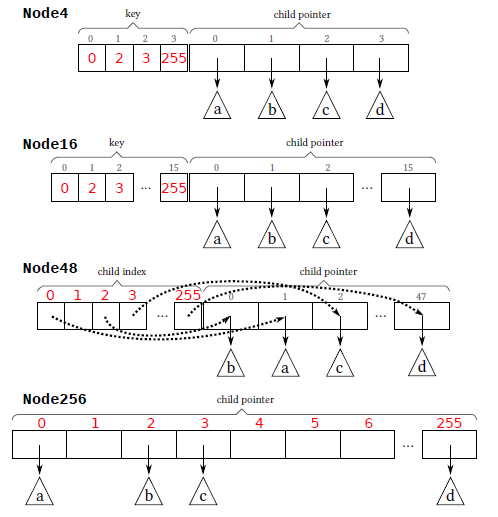
\includegraphics[width=0.5\textwidth]{figure_4.png}
	\caption{Inner nodes of ART. The partial keys 0, 2, 3, and 255 are mapped to the subtrees a, b, c, and d. Adapted from Leis et al. [4].}
	\label{fig}
\end{figure}
\subsection{VAST}\label{SCM}
% What is from FAST
Yamamuro et al. extended FAST building an index structure called Vector-Advanced and Compressed Structure Tree (VAST) [5]. They adapt the blocking and aligning structure of FAST and add compression of nodes along with improved SIMD usage. In Figure 5, we show the structure of the VAST-Tree including layers and different blocking elements. The top layer $P_{32}$ uses the techniques of FAST with the same SIMD, cache line and page blocking with 32 bit keys.

% Block compression
In order to decrease the size of the index structure to better fit into main memory, the middle and bottom layers use compressed nodes. In the layer $P_{16}$ the 32 bit keys of each node are compressed to 16 bit keys using lossy compression. Analogue, in $P_8$ the keys are compressed to 8 bit with lossy compression. In the leaf nodes Yamamuro et al. decrease the node size with the lossless compression algorithm \emph{P4Delta}, which a good balance between compression ratio and decompression speed. If an error occurs due to information loss, they present an algorithm for error correction.

% SIMD usage
Along with the other considered index structures, Yamamuro et al. compare multiple keys to one search key with SIMD in the tree traversal. Due to the key compression of nodes, the VAST-Tree compares more keys in parallel than FAST. Additionally, they reduce branch misses with an adapted SIMD usage. They use addition and multiplication operations on the results of a SIMD key comparison, instead of if-then paths, to find the next node in tree traversal.

% Performance
Due to lossy and lossless compression of the majority of nodes, Yamamuro et al. present a 95\% less space consumption of the VAST-Tree compared to a binary tree or FAST. We consider an index with $2^{32}$ keys. They reach up to $6.0$ and $1.24$ times performance increase compared to a binary tree and FAST. Although errors occur due to lossy compression, the error correction does not take a major influence on the traversal speed.

\begin{figure}
	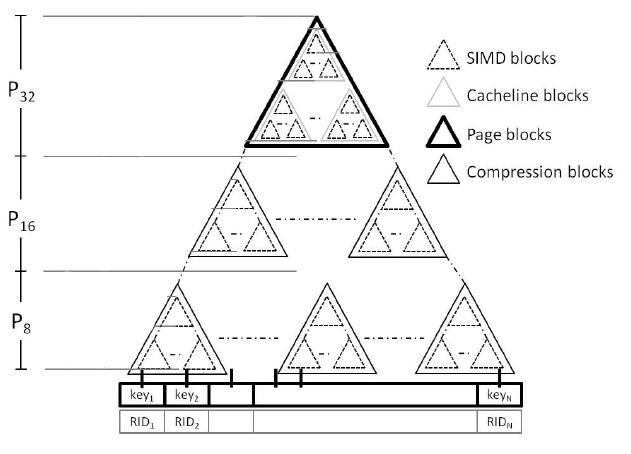
\includegraphics[width=0.5\textwidth]{figure_5.png}
	\caption{An overview of VAST-Tree. The top layer ($P_{32}$) of VAST-Tree uses FAST techniques, and VAST-Tree compresses the middle and the bottom layers ($P_{16}$ and $P_8$) of the trees. Moreover, keys in leaf nodes ($key_1, key_2, ...,	key_N$) are compressed by using lossless compression. Adapted from Yamamuro et al. [5].}
	\label{fig}
\end{figure}

\section{Evaluation}
% What we want to do:
In this section, we present the most important points of index structures that lead to performance decrease. We compare the adaptions made in Seg-Tree, FAST, ART, and VAST to overcome these points and also show differences. We focus on the usage of SIMD within the adapted index structures. 
All considered adaptions have the following points in common:
% In Common:
\begin{itemize}
	\item Keep the key size as small as possible, to compare more keys in parallel
	\item Segmenting tree to blocks for a better usage of SIMD registers and cache lines
	\item SIMD instructions used to compare the search key with multiple keys of the index
\end{itemize}

% Small keys, to compare more in parallel
Before looking at the differences, we go into detail for each entry of the list. At first, keeping the key size as small as possible speeds up the search performance, because more keys can be compared with a single SIMD instruction. Additionally, the smaller the keys are, the more keys fit into the cache line. Since tries or radix trees, depending on their span, have small chunks of the search key in each node, SIMD speeds up the comparison performance by a considerable factor. If keys are stored completely in one node, like in Seg-Tree and FAST, Yamamuro et al. show that compression of keys results in better search performance [5].

% Segmenting the tree
Secondly, all adapted index structures are segmented into blocks (we consider each node of Seg-Tree, a k-ary search tree, also as block). 

% SIMD usage
Segmenting the index structure is important to reach a better performance increase with SIMD instructions. Since the data for a SIMD operation has to be stored sequentially in main memory, a good segmenting and blocking strategy is necessary. In Section 2, we present the vertical vectorization as alternative to horizontal vectorization. Due to the necessary of sequential store of the data in main memory, comparing a different search key per vector lane is not applicable for SIMD instructions in tree traversal. Therefore, all considered adaptions use horizontal vectorization. 

% Decreasing Branch misses with addition/multiplication operations

% Performance comparison
Differences:
\begin{itemize}
	\item Node compression in VAST, Path compression in ART and K-ary seg trie
	\item FAST and K-ary trees readonly to improve traversal, ART and FAST adapt insert too
	\item FAST uses and K-ary trees will use GPU calculation instead of CPU
\end{itemize}

Why performance can not be compared in a useful way...
performance issues:
\begin{itemize}
	\item Seg-Tree: 
\end{itemize}
\section{Related Work}
TODO:
\begin{itemize}
	\item ART and VAST compared to FAST??
	\item Ideas and implementations of the adapted trees already in III...
	\item KD-Tree with SIMD
\end{itemize}

\section{Conclusion}

\section{Future work}
- Using k-ary search in FAST/VAST
- Looking in detail to the decrease of branch misses using addition/multiplication operations and SIMD, combine with k-ary search

%Open questions, use SIMD for tree creation/updates instead of only for traversal
\begin{thebibliography}{00}
\bibitem{b1}Mohammad Suaib, Abel Palaty and Kumar Sambhav Pandey, ``Architecture of SIMD Type Vector Processor'' in International Journal of Computer Applications (0975 - 8887) Volume 20 No.4, April 2011.
\bibitem{b2} Jingren Zhou and Kenneth A. Ross  ``Implementing Database Operations Using SIMD Instructions'' in ACM S1GMOD '2002 June 4-6, Madison, Wisconsin, USA
\bibitem{b3} Steffen Zeuch, Frank Huber and Johann-Christoph Freytag  ``Adapting Tree Structures for Processing with SIMD Instructions'' in Proc. 17th International Conference on Extending Database Technology (EDBT), March 24-28, 2014, Athens, Greece
\bibitem{b4} Viktor Leis, Alfons Kemper and Thomas Neumann ``The Adaptive Radix Tree: ARTful Indexing for Main-Memory Databases''
\bibitem{b5} Takeshi Yamamuro, Makoto Onizuka,Toshio Hitaka, and Masashi Yamamuro ``VAST-Tree: A Vector-Advanced and Compressed Structure for Massive Data Tree Traversal'' in EDBT 2012, March 26-30, 2012, Berlin, Germany.
\bibitem{b6} Changkyu Kim, Jatin Chhugani, Nadathur Satish, Eric Sedlar, Anthony D. Nguyen,
Tim Kaldewey, Victor W. Lee, Scott A. Brandt and Pradeep Dubey ``FAST: Fast Architecture Sensitive Tree Search
on Modern CPUs and GPUs'' in SIGMOD’10, June 6-11, 2010, Indianapolis, Indiana, USA.
\bibitem{b7}Orestis Polychroniou, Arun Raghavan and Kenneth A. Ross, ``Rethinking SIMD Vectorization for In-Memory Databases'' in SIGMOD’15, May 31-June 4, 2015, Melbourne, Victoria, Australia.
\end{thebibliography}

\end{document}
